\documentclass[aps,prl,showpacs,amsmath,amssymb,superscriptaddress,reprint,10pt]{revtex4-1}
\usepackage{bm}
\usepackage{graphicx}
\usepackage{xcolor}
\usepackage{url}
\usepackage[normalem]{ulem}
\usepackage{times}
\usepackage{bbm}
\usepackage{mathrsfs} %Fancy letters 
%\usepackage[colorlinks,linkcolor=blue,anchorcolor=blue,citecolor=blue,filecolor=blue,menucolor=blue,urlcolor=blue]{hyperref}
\usepackage[colorlinks=true,breaklinks=true,allcolors=blue]{hyperref}

\definecolor{lorenzo}{rgb}{1,.4,.3}
\newcommand{\lp}[1]{{\color{lorenzo} #1}}
\definecolor{analabha}{rgb}{0,0,1}
\newcommand{\ar}[1]{{\color{analabha} #1}}
\definecolor{michael}{rgb}{0,.8,.5}
\newcommand{\mk}[1]{{\color{michael} #1}}

\newcommand\Sphere{{\mathbbm{S}}}
\newcommand\NN{{\mathbbm{N}}}
\newcommand\ZZ{{\mathbbm{Z}}}
\newcommand\RR{{\mathbbm{R}}}
\newcommand\CC{{\mathbbm{C}}}
\newcommand\id{{\mathbbm{1}}}

\newcommand\dd{{\mathrm{d}}}
\newcommand\ee{{\mathrm{e}}}
\newcommand\ii{{\mathrm{i}}}
\newcommand{\mvec}[1]{\boldsymbol #1}
\newcommand{\Com}[2]{\left[{#1},{#2}\right]}

\DeclareMathOperator{\Tr}{{Tr}}


%\allowdisplaybreaks

\begin{document}

\title{Simulation of Quantum Spin Dynamics by Phase Space Sampling of BBGKY Trajectories}  

\author{Lorenzo Pucci} 
\affiliation{National Institute for Theoretical Physics (NITheP), Stellenbosch 7600, South Africa} 

\author{Analabha Roy} 
\affiliation{National Institute for Theoretical Physics (NITheP), Stellenbosch 7600, South Africa} 

\author{Michael Kastner} 
%\email{kastner@sun.ac.za} 
\affiliation{National Institute for Theoretical Physics (NITheP), Stellenbosch 7600, South Africa} 
\affiliation{Institute of Theoretical Physics,  University of Stellenbosch, Stellenbosch 7600, South Africa}

\date{\today}

\begin{abstract}
A numerical method, suitable for the simulation of the time evolution of quantum spin models of arbitrary lattice dimension, is presented. The method combines sampling of the Wigner function with evolution equations as obtained from the Bogoliubov-Born-Green-Kirkwood-Yvon (BBGKY) hierarchy. Going to higher orders of the BBGKY hierarchy allows for a systematic refinement of the method. Quantum correlations are treated through both, the Wigner function sampling and the BBGKY evolution, bringing about a significantly improved accuracy when calculating correlation functions. The method is particularly suitable for long-range interacting systems, and we demonstrate its power by comparing with exact results as well as other numerical methods. As an application we compute spin squeezing in a two-dimensional lattice with power-law interactions, as measured in recent ion trap experiments.
\end{abstract}

%\pacs{05.70.Ln, 05.20.-y, 05.30.-d, 05.50.+q} 

\maketitle 
%------------------------------------------------


With the development of highly controllable platforms for quantum simulation, experimental realizations of a variety of, among others, spin lattice models have become available \cite{Simon_etal11,*Struck_etal11,*Labuhn,Britton_etal12,Schauss_etal12,*Islam_etal13,*dePaz_etal13,*Yan_etal13,*Jurcevic_etal14,*Richerme_etal14}. Many of these realization allow for the preparation of initial states far from equilibrium, and the subsequent time evolution according to a given spin Hamiltonian. For one-dimensional lattices, reliable numerical methods, often based on matrix product states, are available to complement the experimental efforts, at least up to intermediate time scales \cite{Schollwoeck11}. In two- and higher-dimensional lattices, computational methods for strongly interacting quantum systems out of equilibrium are scarce, and further development of simulation methods is much needed.

In this Letter we develop a novel simulation method by combining phase space sampling of the initial state with a systematic semi-classical expansion based on the BBGKY hierarchy. The sampling scheme is inspired by a discrete Wigner representation for spin systems as introduced by Wootters \cite{Wootters87}, and was recently used in the context of dynamical simulations by Schachenmayer {\em et al.} \cite{Schachenmayer_etal15}. This scheme can to some extend account for quantum correlations, but it neglects much of their dynamics. To improve on this aspect, we combine the sampling with a systematic way of deriving time evolution equations for arbitrary $n$-point correlations, based on the BBGKY hierarchy of time evolution equations for reduced density operators \cite{Bonitz}. In the past decade or so, BBGKY techniques have been successfully applied to classical systems with long-range interactions \cite{BouchetDauxois05,*Nardini_etal12}, where the error made when truncating the infinite hierarchy of equations 
is known to vanish with increasing system size \cite{BraunHepp77}. For this reason we expect the phase space sampling method for BBGKY trajectories to be particularly suitable for many-particle systems with long-range interactions. Benchmarking against exactly solvable models confirms this expectation, and indicates that our method is a candidate for the most accurate dynamical simulation technique on the market for higher-dimensional spin models with long-range interactions.


{\em Discrete Wigner representation.---}For concreteness we use Wootters's representation of a spin-$1/2$ degree of freedom, but higher spin quantum numbers can be treated along similar lines \cite{Wootters87}. Starting point is a discrete phase space $\Gamma=\left\{(0,0),(0,1),(1,0),(1,1)\right\}$ consisting of four points is introduced, to each of which a 3-vector is associated, $\mvec{r}_{(0,0)}=(1,1,1)$, $\mvec{r}_{(0,1)}=(-1,-1,1)$, $\mvec{r}_{(1,0)}=(1,-1,-1)$, and $\mvec{r}_{(1,1)}=(-1,1,-1)$. To each phase space point $\alpha\in\Gamma$ one assigns a so-called phase space operator
\begin{equation}\label{e:Aalpha}
A_\alpha = \tfrac{1}{2}(\id+\mvec{r}_\alpha\cdot\mvec{\sigma}),
\end{equation}
where $\mvec{\sigma}=\left(\sigma^x,\sigma^y,\sigma^z\right)$ is the vector of Pauli operators. A density operator $\rho$ on $\CC^2$ can then be written  as a linear combination of phase space operators,
\begin{equation}
\rho=\sum_{\alpha\in\Gamma}w_\alpha A_\alpha,
\end{equation}
where the weights $w_\alpha=\Tr(\rho A_\alpha)/2$ form a quasi-probability distribution analogous to the Wigner function for continuous degrees of freedom \cite{Wootters87}. For $N$ spin-$1/2$ degrees of freedom and assuming a product (initial) state, such a phase space representation generalizes to
\begin{equation}
\rho_0=\sum_{\alpha_1,\dotsc,\alpha_N\in\Gamma}w_{\alpha_1}\cdots w_{\alpha_N}A_{\alpha_1}\otimes\cdots\otimes A_{\alpha_N}.
\end{equation}
If the weights $w_i$ calculated from $\rho_0$ happen to be all nonnegative, we can sample from this initial state by drawing $N$-spin phase space points $\mvec{\alpha}=(\alpha_1,\dotsc,\alpha_N)\in\Gamma^N$ according to the probability distribution $w_{\alpha_1}\cdots w_{\alpha_N}$. In practice we use a slightly different, and superior, sampling scheme, which is detailed in the Supplemental Material. This sampling, which is inspired by Ref.~\cite{Schachenmayer_etal15}, is the first main ingredient of our numerical scheme.

{\em BBGKY evolution equations.---}As a second ingredient we derive semi-classical evolution equations with which to propagate the sampled initial phase space points. To this purpose we write the time-evolution of the density operator as
\begin{equation}\label{e:rho_t}
\rho(t)=\sum_{\alpha_1,\dotsc,\alpha_N\in\Gamma}w_{\alpha_1}\cdots w_{\alpha_N} \mathscr{A}_{1\dotsc N}^{\alpha_1\dotsc\alpha_N}(t),
\end{equation}
where the operators $\mathscr{A}_{1\dotsc N}^{\alpha_1\dotsc\alpha_N}(t)=\ee^{-\ii Ht}A_{\alpha_i}\otimes\cdots\otimes A_{\alpha_N}\ee^{\ii Ht}$  have unit trace and satisfy a Liouville-von Neumann equation,
\begin{equation}\label{VNeqdWA}
\ii\partial_t \mathscr{A}_{1\dotsc N}^{\alpha_1\dotsc\alpha_N} = \Com{H}{\mathscr{A}_{1\dotsc N}^{\alpha_1\dotsc\alpha_N}}.
\end{equation}
Unlike Ref.~\cite{Schachenmayer_etal15}, we chose to write the time evolution \eqref{e:rho_t} in the Schr\"odinger picture, as this naturally leads to the systematic approximation scheme introduced in the following.

While the operators $\mathscr{A}_{1\dotsc N}^{\alpha_1\dotsc\alpha_N}$ are in general not positive definite and therefore do not qualify as density operators, reduced $\mathscr{A}$-operators (analogous to reduced density operators) can be defined by tracing out parts of the system,
\begin{equation}
\mathscr{A}_i^{\alpha_1\dotsc\alpha_N}=\Tr_{\not{\,i}} \mathscr{A}_{1\dotsc N}^{\alpha_1\dotsc\alpha_N},\quad \mathscr{A}_{ij}^{\alpha_1\dotsc\alpha_N}=\Tr_{\not{\,i}\not{\,j}} \mathscr{A}_{1\dotsc N}^{\alpha_1\dotsc\alpha_N}.
\end{equation}
Here, $\Tr_{\not{\,i}}$ denotes a partial trace over all of the tensor product Hilbert space except for the factor associated with spin $i$. In the spirit of the BBGKY hierarchy for reduced density operators \cite{Bonitz}, the time evolution \eqref{VNeqdWA} for a general Hamiltonian
\begin{equation}\label{e:Hgen}
H_{1\dotsc N} = \sum_i H_i + \sum_{i<j}H_{ij}
\end{equation}
with on-site and pair interactions can be recast in the form of a hierarchy of equations for the $n$-spin reduced $\mathscr{A}$-operators (see Supplemental Material for details). For the long-range interacting systems we intend to simulate, we expect deviations from mean-field to be small. This suggests to separate the $\mathscr{A}$-operators into product and correlated parts by means of a cluster expansion,
\begin{subequations}
\begin{align}
\mathscr{A}_{ij}&=\mathscr{A}_i \mathscr{A}_j+\mathscr{C}_{ij},\label{e:cluster1}\\
\mathscr{A}_{ijk}&=\mathscr{A}_i \mathscr{A}_j \mathscr{A}_k + \mathscr{A}_i \mathscr{C}_{jk} + \mathscr{A}_j \mathscr{C}_{ik} + \mathscr{A}_k \mathscr{C}_{ij} + \mathscr{C}_{ijk},\label{e:cluster2}
\end{align}
\end{subequations}
and similarly for higher orders. Superscripts $\alpha_1\dotsc\alpha_N$ of $\mathscr{A}$ and $\mathscr{C}$ are for the moment suppressed. In terms of these operators the first two equations of the BBGKY hierarchy read
\begin{subequations}
\begin{align}
\ii\partial_t \mathscr{A}_i=&\Com{H_i}{\mathscr{A}_i}+\sum_{k\neq i}\Tr\Com{H_{ik}}{\mathscr{C}_{ik}+\mathscr{A}_i \mathscr{A}_k}\label{e:1st_order}\\
\ii\partial_t \mathscr{C}_{ij}=&\Com{H_i+H_j+H_i^\text{H}+H_j^\text{H}}{\mathscr{C}_{ij}}+\Com{H_{ij}}{\mathscr{C}_{ij}+\mathscr{A}_i \mathscr{A}_j}\nonumber\\
&+\sum_{k\neq i,j}\left(\Tr_k\Com{H_{ik}}{\mathscr{A}_i \mathscr{C}_{jk}}+\Tr_k\Com{H_{jk}}{\mathscr{A}_j \mathscr{C}_{ik}}\right)\nonumber\\
&-\mathscr{A}_i\Tr_i\Com{H_{ij}}{\mathscr{C}_{ij}+\mathscr{A}_i \mathscr{A}_j}\nonumber\\
&-\mathscr{A}_j\Tr_j\Com{H_{ij}}{\mathscr{C}_{ij}+\mathscr{A}_i \mathscr{A}_j}\label{e:2nd_order}
\end{align}
\end{subequations}
with the Hartree operator
\begin{equation}
 H_i^\text{H}=\sum_{k\neq i,j}\Tr_k\left(H_{ik} \mathscr{A}_k\right).
\end{equation}
In \eqref{e:2nd_order} we have neglected the 3-spin correlations $\mathscr{C}_{ijk}$, and this approximation is expected to be good for intermediate times and sufficiently long-ranged interactions. Improving this scheme systematically by truncating the BBGKY hierarchy at higher order is straightforward, at a numerical cost that scales like $\mathscr{O}\left(N^n\right)$ with system size $N$ and truncation order $n$. If we were to neglect also the 2-spin correlations $\mathscr{C}_{ij}$ in \eqref{e:1st_order}, and disregard \eqref{e:2nd_order} entirely, we would recover the time evolution equations used in Ref.~\cite{Schachenmayer_etal15}.

Next, we represent the $\mathscr{A}$- and $\mathscr{C}$-operators in the basis of Pauli operators,
\begin{subequations}
\begin{align}
\mathscr{A}_i &= \tfrac{1}{2}\left(\id_i+\mvec{a}_i\cdot\mvec{\sigma}_i\right),\label{e:Aexp}\\
%\mathscr{A}_i =& \frac{1}{2}\left(\id_i+\sum_{\mu\in\{x,y,z\}}a_i^\mu\sigma_i^\nu\right),\\
\mathscr{C}_{ij} &= \tfrac{1}{4}\sum_{\mu,\nu\in\{x,y,z\}}c_{ij}^{\mu\nu}\sigma_i^\mu\sigma_j^\nu.\label{e:Cexp}
\end{align}
\end{subequations}
Inserting these expansions into the BBGKY equations \eqref{e:1st_order} and \eqref{e:2nd_order}, we obtain time evolution equations for the expansion coefficients $a_i^\mu$ and $c_{ij}^{\mu\nu}$ \cite{PaskauskasKastner12}; see the Supplemental Material for a derivation of the somewhat lengthy equations. This set of $3N(3N-2)/2$ coupled ordinary differential equations is the second main ingredient of our simulation method.

In summary, the simulation method consists of the following steps. (1) Sample phase space points $\mvec{\alpha}$ from the probability distribution $w_{\alpha_1}\cdots w_{\alpha_N}=2^{-N}\Tr\left[\rho_0 \mathscr{A}_{1\dotsc N}^{\alpha_1\dotsc\alpha_N}(0)\right]$ of the initial state $\rho_0$. (2) Compute the corresponding initial values of the Pauli expansion coefficients $a_i^\mu=\Tr\left(\sigma_i^\mu \mathscr{A}_{1\dotsc N}^{\alpha_1\dotsc\alpha_N}\right)$. The correlation coefficients $c_{ij}^{\mu\nu}$ are initially zero for a product state. (3) Time-evolve $a_i^\mu$ and $c_{ij}^{\mu\nu}$ according to the semi-classical equations of motion \eqref{e:1st_order_param}--\eqref{e:2nd_order_param} in the Supplemental Material. (4) Calculate expectation values of 1- or 2-spin functions,
%\begin{equation}
%\left\langle\sigma_i^\mu\right\rangle \approx \sum_{\mvec{\alpha}}a_i^\mu,\qquad
%\left\langle\sigma_i^\mu\sigma_j^\nu\right\rangle - \left\langle\sigma_i^\mu\right\rangle\left\langle\sigma_j^\nu\right\rangle \approx \sum_{\mvec{\alpha}}c_{ij}^{\mu\nu},
%\end{equation}
\begin{subequations}
\begin{align}
\left\langle\sigma_i^\mu\right\rangle =& \sum_{\mvec{\alpha}\in\Gamma^N}w_{\alpha_1}\cdots w_{\alpha_N} a_i^\mu \approx \sum_{\mvec{\alpha}\in S_n}a_i^\mu,\label{e:1spin}\\
\left\langle\sigma_i^\mu\sigma_j^\nu\right\rangle - \left\langle\sigma_i^\mu\right\rangle\left\langle\sigma_j^\nu\right\rangle =& \sum_{\mvec{\alpha}\in\Gamma^N}w_{\alpha_1}\cdots w_{\alpha_N} c_{ij}^{\mu\nu} \approx \sum_{\mvec{\alpha}\in S_n}c_{ij}^{\mu\nu},\label{e:2spin}
\end{align}
\end{subequations}
where $S_n=\left\{\mvec{\alpha}^{(1)},\dots,\mvec{\alpha}^{(n)}\right\}$ is a sample of $n$ phase space points drawn from the probability distribution $w_{\alpha_1}\cdots w_{\alpha_N}$.


{\em Benchmarking.---}To test the accuracy of the simulation method, we benchmark the results against exact analytic and numeric calculations for simple one-dimensional model systems. The improved performance of our method is highlighted by comparing to the results of Schachenmayer, Pikovski, and Rey \cite{Schachenmayer_etal15} (abbreviated to SPR in the following).

The first test case is the quantum Ising chain with long-range interactions,
\begin{equation}\label{e:Ising}
H=-J\sum_{i\neq j}\frac{\sigma_i^z\sigma_j^z}{|i-j|^\alpha} - \mvec{h}\cdot\sum_i\mvec{\sigma}_i,
\end{equation}
where $J$ is a coupling constant and $\mvec{h}$ the magnetic field vector. The exponent $\alpha\geq0$ controls the range of the interactions, and open boundary conditions are used. In the case of a longitudinal magnetic field $\mvec{h}=(0,0,h)$, exact analytic results are known for the time-evolution of 1-spin \cite{Emch66,*Radin70,*Kastner11,*Kastner12} and 2-spin functions \cite{vdWorm_etal13,*FossFeigHazzardBollingerRey13,*KastnerVdWorm}. In the Supplemental Material we show that, for this and also more general models, the middle equations in \eqref{e:1spin} and \eqref{e:2spin} agree with the exact analytic solution, and hence the estimates on the right-hand side of those equations become exact in the limit of large sample size. In this sense, our method is numerically exact for the Ising model in a longitudinal field. A comparison with the method of SPR, which shows deviations from the exact result, is shown in Fig.~\ref{f:Ising}.

\begin{figure}\centering
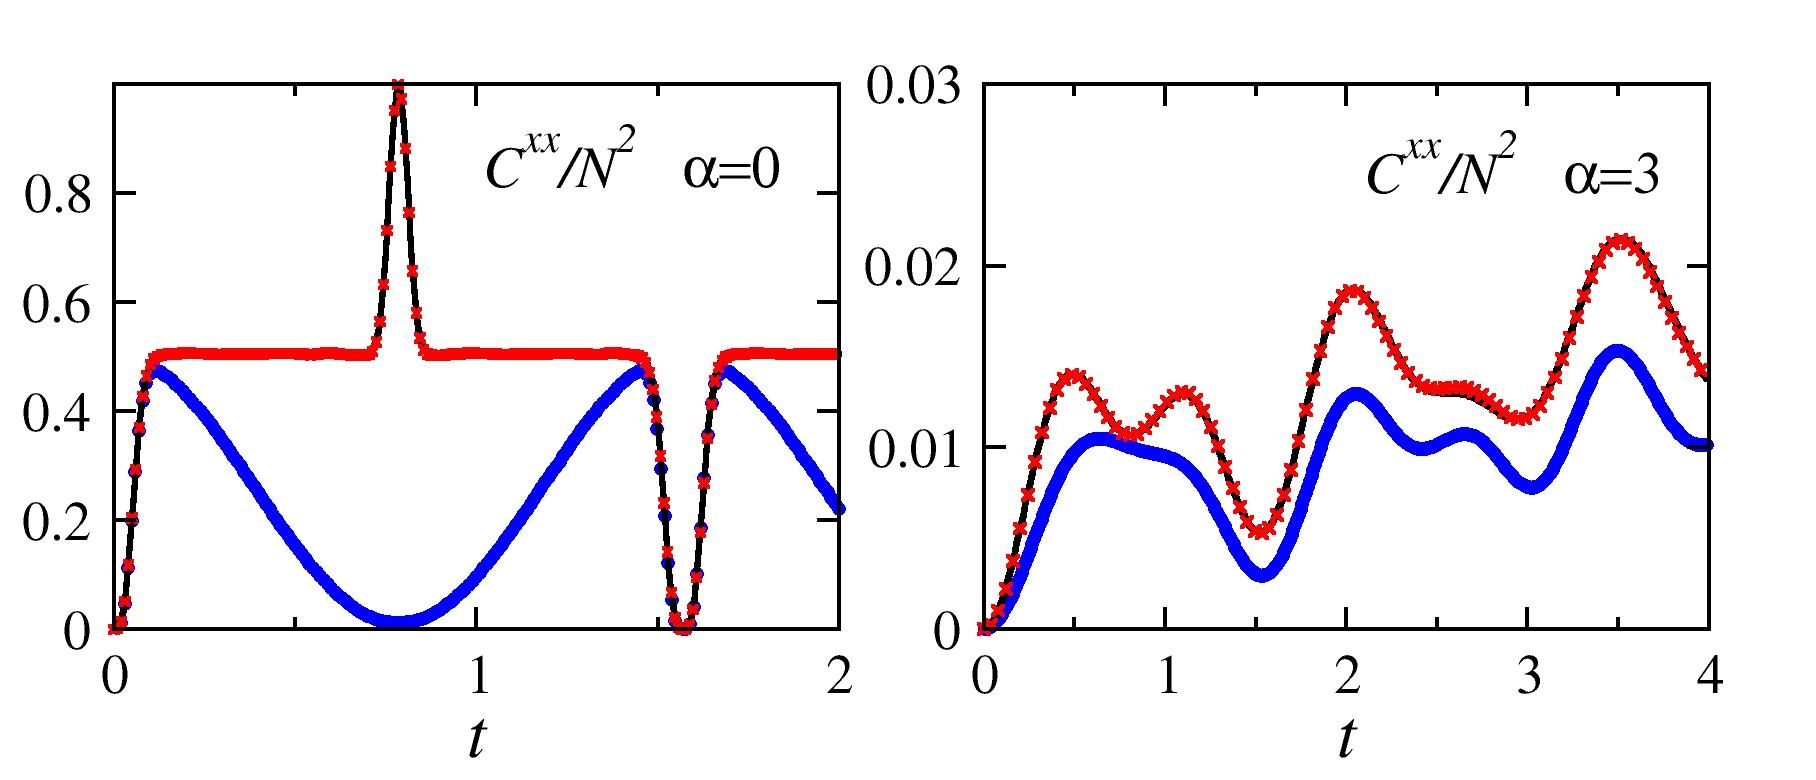
\includegraphics[width=\linewidth]{./Ising_Schach_N100_alph_0_3_nt10000.jpg}
\caption{\label{f:Ising}%
Time evolution of total correlations $C^{xx}=\sum_{i,j}\langle\left\{\sigma_i^x,\sigma_j^x\right\}\rangle/2$ (where the curly brackets denote an anticommutator) for a long-range Ising chain of $100$ sites in a longitudinal field of strength $h=0$ with long-range exponent $\alpha=0$ (left) and $\alpha=3$ (right). As shown analytically in the Supplemental Material, our method recovers the exact solution (black) in the limit of an infinite sample. The only error is therefore of a statistical nature due to the finite sample size $n=10000$ (red crosses). The method of SPR (blue dots) shows systematic deviations from the exact result.
}%
\end{figure}

A magnetic field $\mvec{h}=(h,0,0)$ in \eqref{e:Ising} results in a quantum Ising chain with long-range interactions in a transverse magnetic field, and no analytic solution is known in this case. We calculated 2-spin correlation functions, and also the spin squeezing parameter
\begin{equation}\label{e:spinsqueezing}
\xi = \sqrt{N}\min_{\mvec{n}\perp\langle\mvec{S}\rangle}\frac{\sqrt{\langle(\mvec{S}\cdot\mvec{n})^2\rangle - \langle\mvec{S}\cdot\mvec{n}\rangle^2}}{|\langle\mvec{S}\rangle||\mvec{n}|}
\end{equation}
where $\mvec{S}=\sum_i \mvec{\sigma}_i$, a quantity that can be measured for example in trapped-ion realizations of long-range interacting spin models. A comparison to exact diagonalization results for a chain of 11 sites, and also to the method of SPR, is shown in Fig.~\ref{f:TFIM}. For the chosen parameter values (specified in the figure caption) the spin squeezing shows pronounced spikes at certain times, which are captured by our method. From theoretical arguments we expect the approximation error to become smaller with increasing system size for exponents $\alpha$ smaller than the lattice dimension. 

\begin{figure}\centering
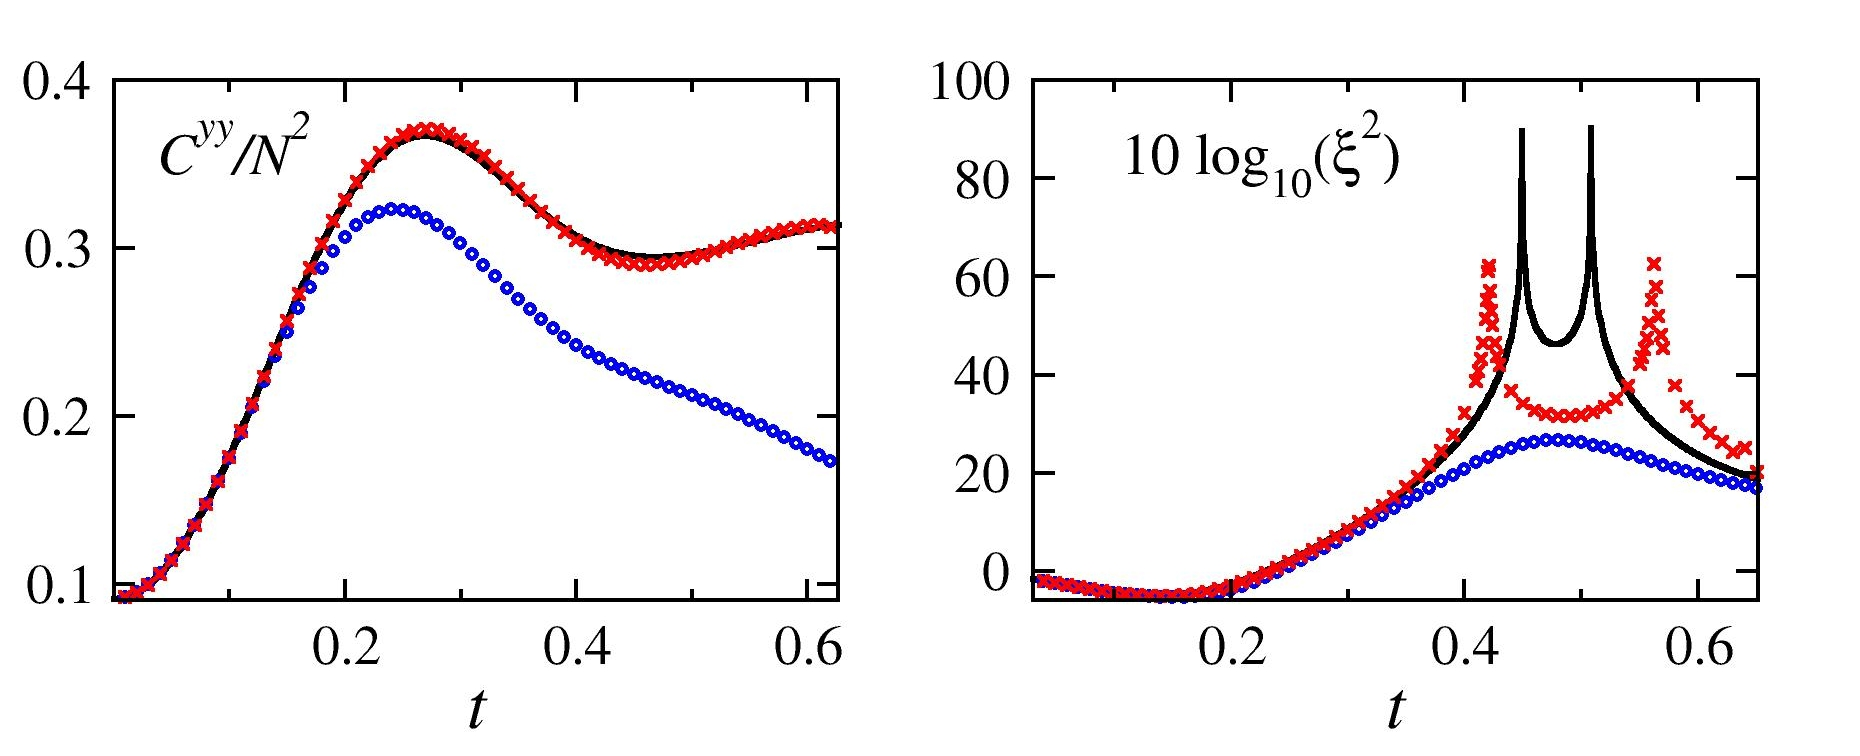
\includegraphics[width=\linewidth]{./Jz1hx1_Schach_alph05_N11_nt500000.jpg}
\caption{\label{f:TFIM}%
Time evolution of a long-range Ising chain of 11 sites with $\alpha=1/2$ in a transverse field of strength $h=1$. We compare exact diagonalization results (black line), the method of SPR (blue dots), and our method (red crosses) for sample sizes $n=5\times10^5$. Left: Total correlations $C^{yy}$. Right: Decibel spin squeezing as obtained from \eqref{e:spinsqueezing}. While not an exact match, our method captures the sharp spikes in the spin squeezing.
}%
\end{figure}

For further benchmarking, we consider the quantum $XX$ chain with long-range interactions,
\begin{equation}\label{e:XY}
H=-J\sum_{i\neq j}\frac{\sigma_i^x\sigma_j^x+\sigma_i^y\sigma_j^y}{|i-j|^\alpha}.
\end{equation}
Here we simulate chains of 100 sites and compare to numerical results from density matrix renormalization group (DMRG) calculations. As shown in Fig.~\ref{f:XX}, correlations and spin squeezing are obtained by our method with remarkable precision.

\begin{figure}\centering
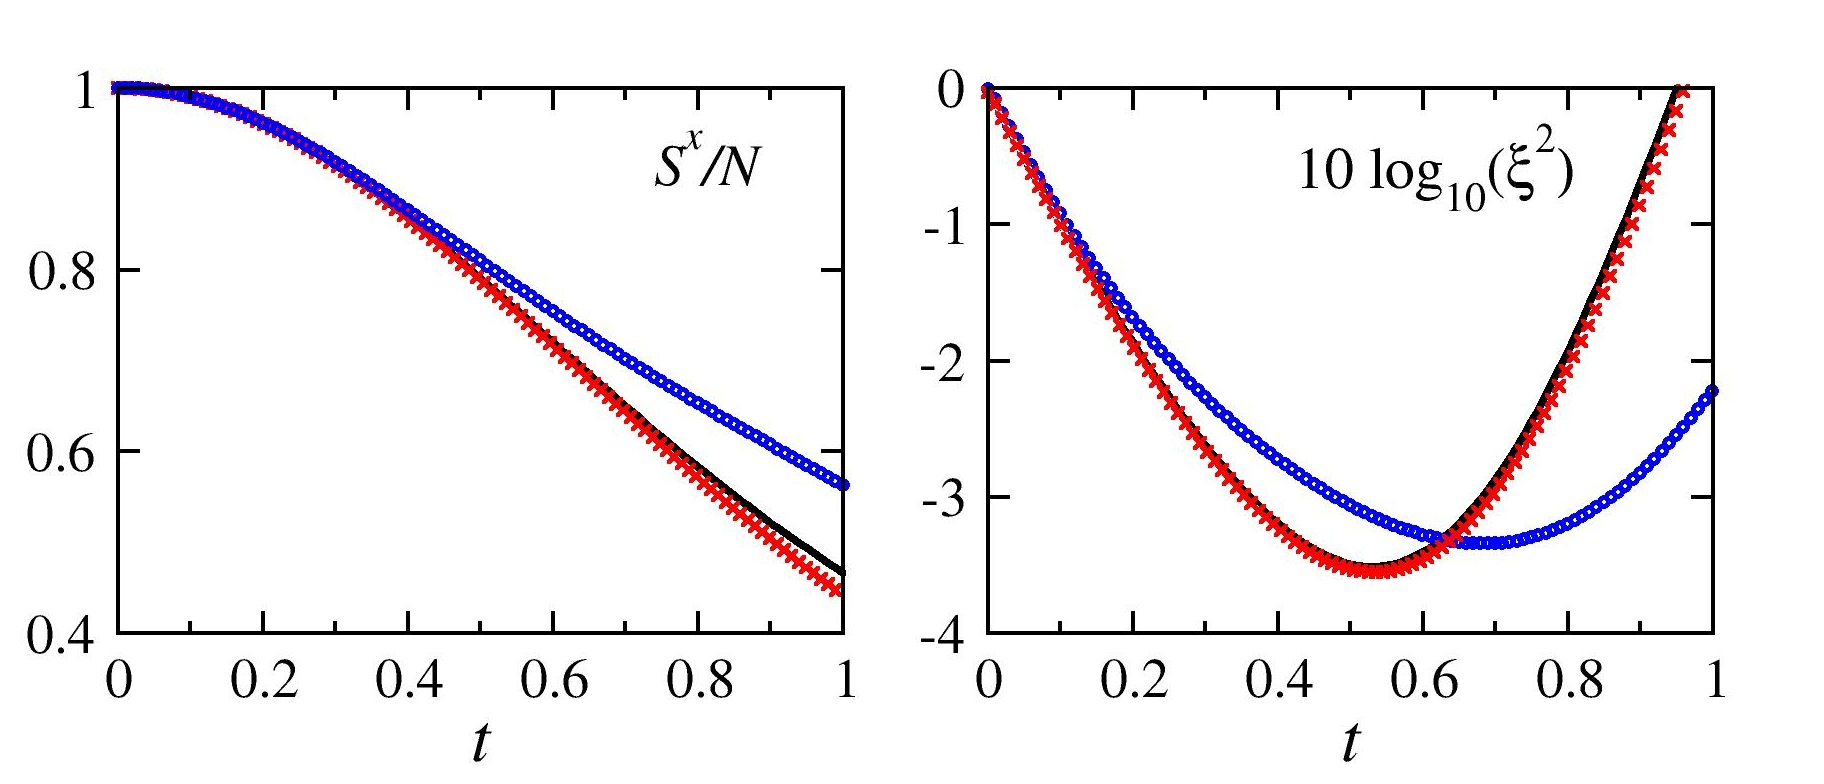
\includegraphics[width=\linewidth]{./Jx05Jy05_Schach_N100_alph3_nt100000.jpg}
\caption{\label{f:XX}%
Time evolution of a long-range $XX$ chain of 100 sites with $\alpha=3$. We compare DMRG results (black line), the method of SPR (blue dots), and our method (red crosses) for sample sizes $n=10^5$. Left: Total spin $S^x=\sum_i\sigma_i^x$. Right: Decibel spin squeezing as obtained from \eqref{e:spinsqueezing}, where the results of our method are virtually indistinguishable from the DMRG data.
}%
\end{figure}


{\em Parameter dependencies.---}\mk{If we have space, otherwise in the Supplemental Material.}


{\em Application to two-dimensional ion crystals.---}While one-dimensional models are suitable for benchmarking our method, it is two- and higher-dimensional systems, where DMRG calculations are not feasible, for which our method is particularly suited. We illustrate its strength by calculating spin squeezing in a transverse-field Ising model on a two-dimensional lattice with hundreds of sites, as it can be emulated with ions in a Penning trap \cite{Britton_etal12}. The Coulomb repulsion between the ions approximately leads to a triangular lattice structure, although distortions occur close to the boundary. Transverse lattice oscillations mediate interactions between hyperfine states of the ions, leading to effective Ising spins with long-range couplings, like in a two-dimensional version of the Hamiltonian \eqref{e:Ising}. The effective magnetic field $\mvec{h}$ in the experiment in \cite{Britton_etal12} can be orientated arbitrarily. For a longitudinal field $\mvec{h}=(0,0,h)$ exact results are available 
and have been used for benchmarking. Here we consider the long-range Ising model with $N=300$ lattice sites in a transverse field $\mvec{h}=(h,0,0)$, where no other good methods are available for calculating how spin squeezing evolves in time. The coupling coefficients $J_{ij}$ are computed numerically by a method outlined in \cite{Britton_etal12}. They decay approximately like $J_{ij}\propto|i-j|^{1/2}$ for the experimentally realistic parameters we have chosen. Numerical results for total correlations and decibel spin squeezing are shown in Fig.~\ref{f:2d}. We believe that computations of this kind will prove useful for locating interesting regimes for future experiments, while experimental data can in turn be used to assess the performance of the numerics.

\begin{figure}\centering
%\includegraphics[width=\linewidth]{./.eps}
\caption{\label{f:2d}%
Time evolution of\dots
}%
\end{figure}


{\em Conclusions.---}We have introduced a numerical method for simulating the time evolution of quantum spin models. The method uses sampling from a discrete phase space representation of the initial state, as recently introduced in \cite{Schachenmayer_etal15}. This ingredient is combined with the time evolution equations \eqref{e:1st_order_param}--\eqref{e:2nd_order_param} obtained from the BBGKY hierarchy, which explicitly account for the time evolution of connected correlations. Benchmarking against exact results confirms that this leads to a significantly improved accuracy when computing correlation functions, as illustrated in Figs.~\ref{f:Ising}--\ref{f:XX}. The numerical cost scales like $\mathscr{O}(N^2)$ with the lattice size $N$. Lattices with $N=\mathscr{O}(10^4)$ are manageable on a personal computer, and $N=\mathscr{O}(10^6)$ should be possible on a supercomputer. Going to higher orders of the BBGKY hierarchy allows for a systematic refinement of the method, but results in a less favorable 
scaling of the numerical cost. While 
the method is presented for spin-$1/2$ degrees of freedom, both, the phase space sampling and the BBGKY time evolution equations can be readily generalized to higher spin quantum numbers.

The method is particularly suitable for long-range interacting systems with small exponents $\alpha$, and can be applied in arbitrary lattice dimension. Of particular interest are applications for two- and higher-dimensional lattices, where established methods like DMRG do not work. An important open question concerns the various sampling schemes discussed in the Supplemental Material. These schemes affect the accuracy of the numerics, but a better understanding is required in order to be able to choose the optimal scheme for a given problem.


%The authors have profited from useful discussion with \dots

%Acknowledge data from J.~ Schachenmayer and J.J.~Bollinger.

M.\,K.\ acknowledges financial support by the National Research Foundation of South Africa via the Incentive Funding and the Competitive Programme for Rated Researchers.


\bibliography{LRLR}

\bigskip

\newpage
%\hbox{}
%\newpage

\begin{center}
{\bf Supplemental Material}  
\end{center}
\vspace{-3mm}
\appendix
\numberwithin{equation}{section}
\numberwithin{figure}{section}


\section{A. Phase space sampling schemes}
\setcounter{section}{1}
\setcounter{equation}{0}
\setcounter{figure}{0}

In the main text of this Letter, a phase space sampling scheme based upon Wootters's discrete phase space representation is described, where the phase space operators \eqref{e:Aalpha} are defined with the 3-vectors
\begin{subequations}
\begin{align}
\mvec{r}_{(0,0)}&=(1,1,1),\label{e:r1}\\
\mvec{r}_{(0,1)}&=(-1,-1,1),\\
\mvec{r}_{(1,0)}&=(1,-1,-1),\\
\mvec{r}_{(1,1)}&=(-1,1,-1).\label{e:r4}
\end{align}
\end{subequations}
However, this choice is not unique. Phase space operators $A_\alpha^\prime=UA_\alpha U^\dagger$ related to the $A_\alpha$ by an overall unitary transform $U$ also have the desired properties of a Wigner representation, and the same holds for phase space operators obtained by a nonsingular linear transformation of the phase space coordinates \cite{Wootters87}. A simple example is provided by the phase point operators
\begin{equation}
A_\alpha^\prime = \tfrac{1}{2}(\id+\mvec{r}_\alpha^\prime\cdot\mvec{\sigma})
\end{equation}
where the 3-vectors
\begin{subequations}
\begin{align}
\mvec{r}_{(0,0)}^\prime&=(1,-1,1),\\
\mvec{r}_{(0,1)}^\prime&=(-1,1,1),\\
\mvec{r}_{(1,0)}^\prime&=(1,1,-1),\\
\mvec{r}_{(1,1)}^\prime&=(-1,-1,-1),
\end{align}
\end{subequations}
are obtained by flipping the sign of the second component in each of the vectors in \eqref{e:r1}--\eqref{e:r4}.

While both these possibilities, as well as the many others, provide valid discrete Wigner representations, the choice of the phase point operators may significantly affect the phase space sampling discussed in the main text. As an example, consider an initial state $\rho_0 = (\id+\sigma^x)/2$ being a $\sigma^x$-eigenstate with eigenvalue $+1$. Using \eqref{e:r1}--\eqref{e:r4} to compute the phase space operators \eqref{e:Aalpha}, one obtains $w_{(0,0)}=w_{(1,0)}=1/2$ and 
$w_{(0,1)}=w_{(1,1)}=0$. Accordingly, in our simulation method one would time-evolve, each with probability $1/2$, either the classical spin vector $a=(1,1,1)$ or $a=(1,-1,-1)$. The $y$- and $z$-components of these two classical spins vectors are fully correlated, but from a physics perspective there is no good reason for them to be so. It would appear more natural to sample from the four classical spin vectors $(1,1,1)$, $(1,1,-1)$, $(1,-1,1)$, and $(1,-1,-1)$, which combines the vectors $\mvec{r}_{(0,0)}$ and $\mvec{r}_{(1,0)}$ from the original set of 3-vectors with $\mvec{r}_{(0,0)}^\prime$ and $\mvec{r}_{(1,0)}^\prime$ from the set of primed ones. Indeed, this is the kind of sampling that was used in \cite{Schachenmayer_etal15}, and it leads to a significant improvement of the numerical results compared to sampling from $\mvec{r}_{(0,0)}$ and $\mvec{r}_{(1,0)}$ only.

Such a sampling from two different phase space representations may appear as going beyond Wootters's discrete Wigner representation, but the validity of this, and many other, generalized sampling schemes can be understood as follows. Splitting the density operator into two parts, $\rho_0=\rho_0/2+\rho_0/2$, we can choose to write the first term in one kind of Wigner representation, and the second in another one,
\begin{equation}\label{e:split1}
\rho_0=\tfrac{1}{2}\sum_{\alpha\in\Gamma}w_\alpha A_\alpha + \tfrac{1}{2}\sum_{\alpha\in\Gamma}w_\alpha^\prime A_\alpha^\prime.
\end{equation} 
For the initial state $\rho_0 = (\id+\sigma^x)/2$, sampling the spin vectors $\mvec{r}_{(0,0)}$, $\mvec{r}_{(1,0)}$, $\mvec{r}_{(0,0)}^\prime$, and $\mvec{r}_{(1,0)}^\prime$ with probabilities of $1/4$ will therefore give a correct sampling.

It is interesting to note that, since $w_\alpha=w_\alpha^\prime$ for all $\alpha$, we can rewrite \eqref{e:split1} as
\begin{equation}\label{e:split2}
\rho_0 = \sum_{\alpha\in\Gamma}w_\alpha \tilde{A}_\alpha
\end{equation}
with
\begin{equation}
\tilde{A}_\alpha = \tfrac{1}{2}\left(A_\alpha + A_\alpha^\prime\right) = \tfrac{1}{2}(\id+\tilde{\mvec{r}}_\alpha\cdot\mvec{\sigma})
\end{equation}
and
\begin{subequations}
\begin{align}
\tilde{\mvec{r}}_{(0,0)}&=(1,0,1),\label{e:rt1}\\
\tilde{\mvec{r}}_{(0,1)}&=(-1,0,1),\\
\tilde{\mvec{r}}_{(1,0)}&=(1,0,-1),\\
\tilde{\mvec{r}}_{(1,1)}&=(-1,0,-1).\label{e:rt4}
\end{align}
\end{subequations}
While the new phase point operators $\tilde{A}_\alpha$ are equivalent to the old ones in being just simple linear combinations, the different choices are crucially different at later times due to the nonlinearity of the equations \eqref{e:1st_order_param}--\eqref{e:2nd_order_param} under which the classical spin vectors \eqref{e:rt1}--\eqref{e:rt4} evolve in time.

Out of the many possible choices of sampling schemes, we have experimented, always for $\rho_0 = (\id+\sigma^x)/2$, with the following sets of vectors to define the phase space operators,
\begin{subequations}
\begin{align}
S_{\text{1-1}}&=\bigl\{\mvec{r}_{(0,0)},\mvec{r}_{(1,0)},\mvec{r}_{(0,0)}^\prime,\mvec{r}_{(1,0)}^\prime\bigr\},\label{e:S11}\\
S_{\text{0-1}}&=\bigl\{\tilde{\mvec{r}}_{(0,0)},\tilde{\mvec{r}}_{(1,0)},\tilde{\mvec{r}}_{(0,0)}^\prime,\tilde{\mvec{r}}_{(1,0)}^\prime\bigr\},\\
S_{\text{all}}&=S_{\text{1-1}}\cup S_{\text{0-1}},\label{e:Sall}
\end{align}
\end{subequations}
where
\begin{equation}
\tilde{\mvec{r}}_{(0,0)}^\prime=(1,1,0),\qquad \tilde{\mvec{r}}_{(1,0)}^\prime=(1,-1,0).
\end{equation}
Numerical results obtained with $S_{\text{1-1}}$, $S_{\text{0-1}}$, and $S_{\text{all}}$ start to differ from each other after some time, as illustrated in Fig.~\ref{f:sampling}. Whether one choice or the other performs better depends on the model studied. Fig.~\ref{f:sampling_2} shows that the sampling scheme performing better does not change by taking different sizes or different $\alpha$'s for the models taken into account. Understanding this dependence, and therefore being able to choose the optimal sampling for a given problem, is an interesting open problem.

\begin{figure}\centering
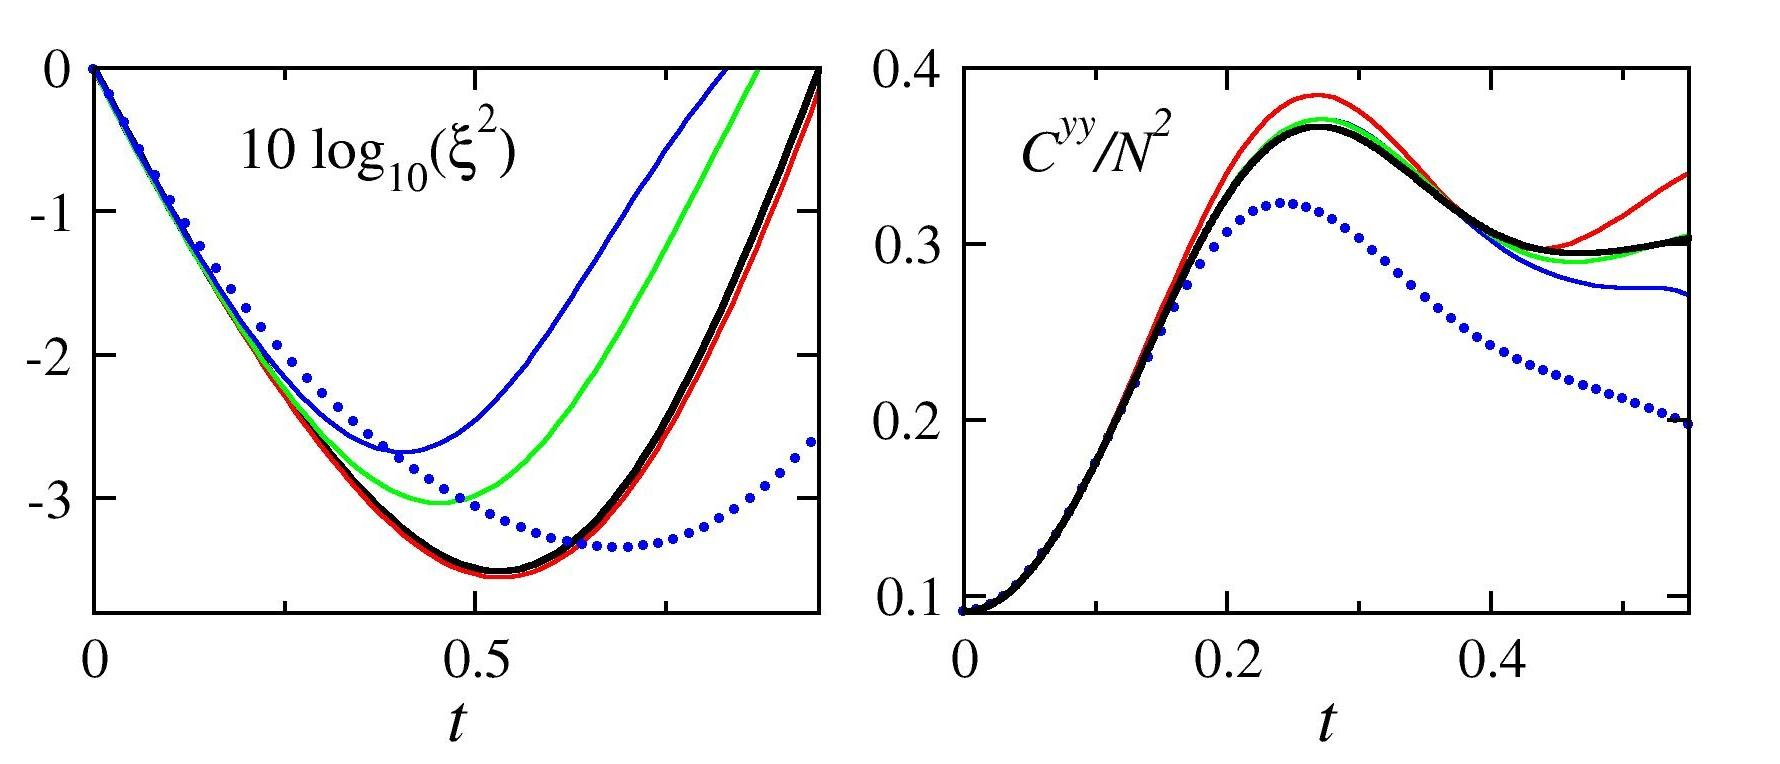
\includegraphics[width=\linewidth]{./XY_TF_compare_samplings.jpg}
\caption{\label{f:sampling}%
Comparison of the different sampling schemes $S_{\text{1-1}}$ (blue), $S_{\text{0-1}}$ (red), and $S_{\text{all}}$ (green) as defined in \eqref{e:S11}--\eqref{e:Sall}, and method of SPR (blue dots). Sample sizes are $n=10^5$ in all cases. Left: Time evolution of the decibel spin squeezing for an $XX$ chain of 100 sites and long-range exponent $\alpha=3$. DMRG results are shown in black. Right: Total correlations $C^{yy}=\sum_{i,j}\left\{\sigma_i^y,\sigma_j^y\right\}/2$ of an Ising chain of 11 sites in a transverse field $\mvec{h}=(1,0,0)$ with long-range exponent $\alpha=1/2$. Results obtained by exact diagonalization are shown in black.
}%
\end{figure}

\begin{figure}\centering
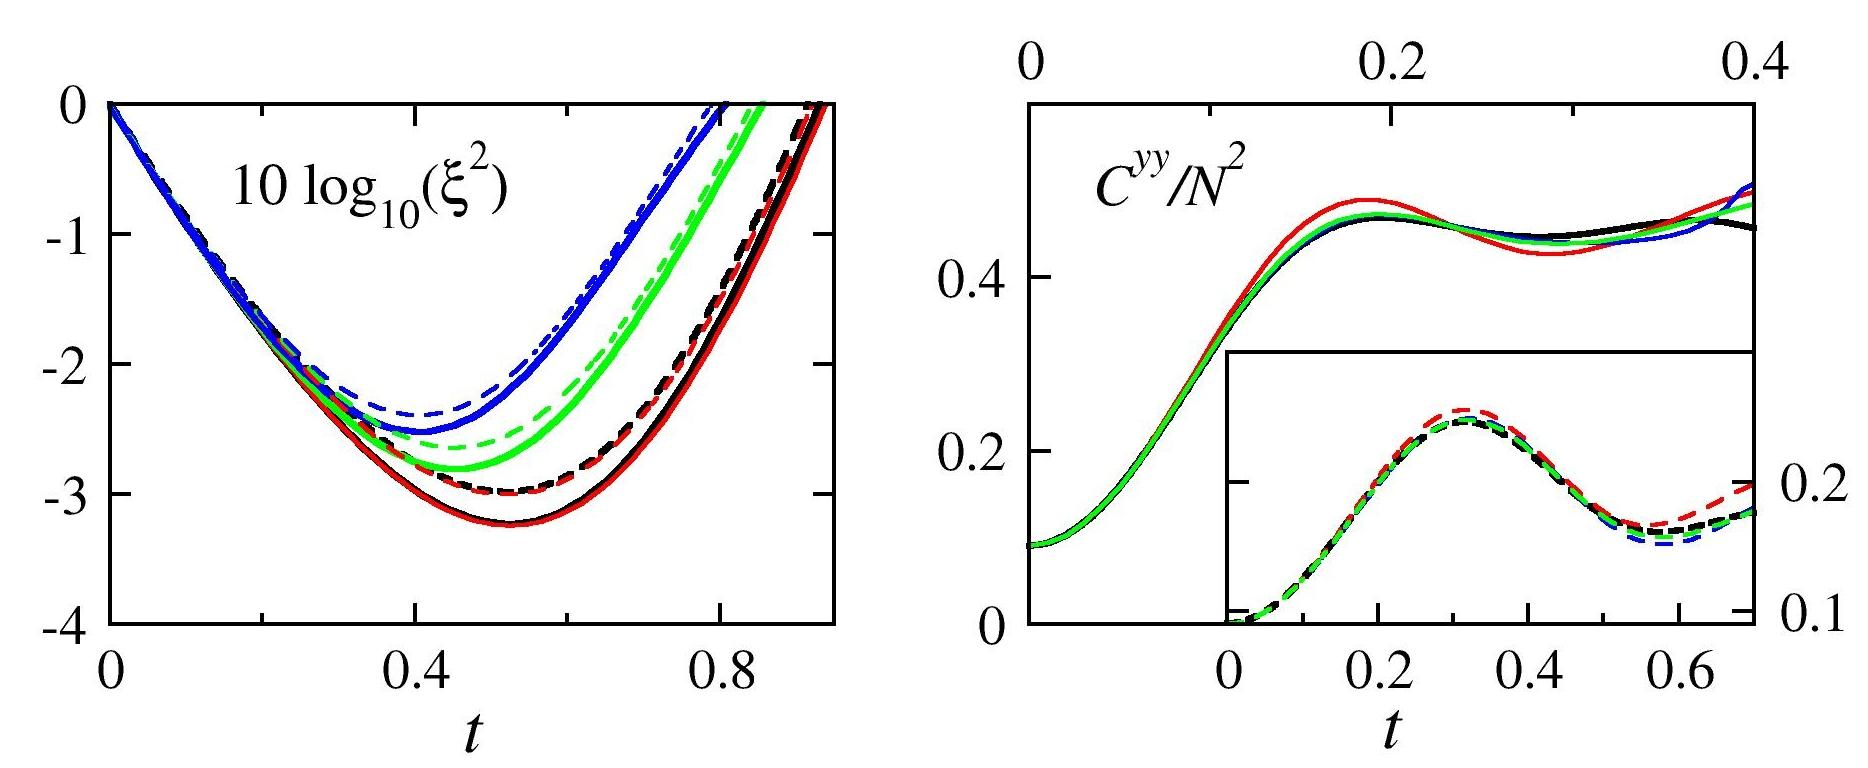
\includegraphics[width=\linewidth]{./benchmark_sizes_XY_alpha_TF.jpg}
\caption{\label{f:sampling_2}%
Comparison of the different sampling schemes $S_{\text{1-1}}$ (blue), $S_{\text{0-1}}$ (red), and $S_{\text{all}}$ (green) as defined in \eqref{e:S11}--\eqref{e:Sall}. Sample sizes are $n=10^5$ in all cases. Left: Time evolution of the decibel spin squeezing for an $XX$ chain of 11 (dashes) and 20 (line) sites and long-range exponent $\alpha=3$ for. DMRG results (line) and those obtained with exact diagonalization (dashes) are shown in black. Right: Total correlations $C^{yy}=\sum_{i,j}\left\{\sigma_i^y,\sigma_j^y\right\}/2$ of an Ising chain of 11 sites in a transverse field $\mvec{h}=(1,0,0)$ with long-range exponent $\alpha=0$ (line) and $\alpha=1$ (dashes). Results obtained with exact diagonalization are shown in black.
}%
\end{figure}

\section{B. Truncated time evolution in Pauli representation}
\setcounter{section}{2}
\setcounter{equation}{0}
\setcounter{figure}{0}

In this section the semi-classical time evolution equations for the Pauli expansion coefficients $a_i^\mu$ and $c_{ij}^{\mu\nu}$ are derived.

Starting from the Liouville-von Neumann equation \eqref{VNeqdWA} with the general Hamiltonian \eqref{e:Hgen} and taking partial traces $\Tr_{\not{\,i}}$, $\Tr_{\not{\,i}\not{\,j}}$, \dots, the BBGKY hierarchy of $N$ coupled differential equations is obtained,
\begin{subequations}
\begin{align}
\ii\partial_t \mathscr{A}_i=&\Com{H_i}{\mathscr{A}_i}+\sum_{k\neq i}\Tr\Com{H_{ik}}{\mathscr{A}_{ik}}\label{e:1st_order_app1}\\
\ii\partial_t \mathscr{A}_{ij}=&\Com{H_i+H_j+H_{ij}}{\mathscr{A}_{ij}}+\sum_{k\neq i,j}\Tr_k\Com{H_{ik}+H_{jk}}{\mathscr{A}_{ijk}}
\label{e:2nd_order_app1}
\end{align}
\end{subequations}
Inserting the cluster expansion \eqref{e:cluster1} and \eqref{e:cluster2} and rearranging terms, the hierarchy takes the form 
\begin{subequations}
\begin{align}
\ii\partial_t \mathscr{A}_i=&\Com{H_i}{\mathscr{A}_i}+\sum_{k\neq i}\Tr\Com{H_{ik}}{\mathscr{C}_{ik}+\mathscr{A}_i \mathscr{A}_k}\label{e:1st_order_app2}\\
\ii\partial_t \mathscr{C}_{ij}=&\Com{H_i+H_j+H_i^\text{H}+H_j^\text{H}}{\mathscr{C}_{ij}}+\Com{H_{ij}}{\mathscr{C}_{ij}+\mathscr{A}_i \mathscr{A}_j}\nonumber\\
&+\sum_{k\neq i,j}\left(\Tr_k\Com{H_{ik}}{\mathscr{A}_i \mathscr{C}_{jk}}+\Tr_k\Com{H_{jk}}{\mathscr{A}_j \mathscr{C}_{ik}}\right)\nonumber\\
&-\mathscr{A}_i\Tr_i\Com{H_{ij}}{\mathscr{C}_{ij}+\mathscr{A}_i \mathscr{A}_j}\nonumber\\
&-\mathscr{A}_j\Tr_j\Com{H_{ij}}{\mathscr{C}_{ij}+\mathscr{A}_i \mathscr{A}_j}\nonumber\\
&+\sum_{k\neq i,j}\left(\Tr_k\Com{H_{ik}}{\mathscr{C}_{ijk}}+\Tr_k\Com{H_{jk}}{\mathscr{C}_{ijk}}\right)
\label{e:2nd_order_app2}
\end{align}
\end{subequations}
Neglecting the 3-spin correlations $\mathscr{C}_{ijk}$, the first two equations of the hierarchy decouple from the rest, as in Eqs.~\eqref{e:1st_order} and \eqref{e:2nd_order} of the main text. Next we use the Pauli representations \eqref{e:Aexp} and \eqref{e:Cexp} of the $\mathscr{A}$- and $\mathscr{C}$-operators, and also expand the Hamiltonian \eqref{e:Hgen} in that basis,
\begin{equation}
H=-\sum_{\mu\in\{x,y,z\}}\sum_{i\neq j}J_{ij}^\mu\sigma_i^\mu\sigma_j^\mu - \mvec{h}\cdot\sum_i\mvec{\sigma}_i
\end{equation}
Inserting the representations into the truncated BBGKY equations \eqref{e:1st_order} and \eqref{e:2nd_order}, one makes use of the orthogonality of the Pauli operators to calculate, by methods similar to the Appendix of Ref.~\cite{PaskauskasKastner12}, the following time evolution equations for the expansion coefficients $a_i^\mu$ and $c_{ij}^{\mu\nu}$ for all $i,j=1,\dotsc,N$ and $\mu,\nu\in\{x,y,z\}$.
\begin{widetext}
\begin{subequations}
\begin{align}
 \frac{1}{2}\partial_t a_i^\mu=&-\sum_{\beta\gamma}\left[\left(h^\beta+\sum_{k\neq i}J_{ik}^\beta a_k^\beta\right)a_i^\gamma+\sum_{k\neq i}J_{ik}^\beta c_{ki}^{\beta\gamma}\right]\varepsilon^{\mu \beta\gamma}\label{e:1st_order_param}\\
\frac{1}{2}\partial_t c_{ij}^{\mu\nu}=&-\sum_{\beta}(J_{ij}^\nu a_i^\beta-J_{ij}^\mu a_j^\beta)\varepsilon^{\mu\nu\beta}\nonumber\\
 &-\sum_{\beta,\gamma}\left[\left(h^\beta+\sum_{k\neq i,j}J_{ik}^\beta a_k^\beta\right)c_{ij}^{\gamma\nu}\varepsilon^{\beta \gamma\mu}+\left(h^\beta+\sum_{k\neq i,j}J_{jk}^\beta a_k^\beta\right) c_{ij}^{\mu \gamma}\varepsilon^{\beta \gamma\nu}\right]\nonumber\\
 &-\sum_{\beta,\gamma}\sum_{k\neq i,j}\left[J_{ik}^\beta a_i^\gamma c_{jk}^{\nu\beta}\varepsilon^{\beta \gamma\mu}+J_{jk}^\beta a_j^\gamma c_{ik}^{\mu\beta}\varepsilon^{\beta \gamma\nu}\right]\nonumber\\
 &+\sum_{\beta,\gamma}J_{ij}^\beta \left[a_i^\mu(c_{ij}^{\beta \gamma}+a_i^\beta a_j^\gamma)\varepsilon^{\beta \gamma b}+a_j^\nu(c_{ij}^{\gamma\beta}+a_i^\gamma a_j^\beta)\varepsilon^{\beta \gamma a}\right].
\label{e:2nd_order_param}
 \end{align}
\end{subequations}
 \end{widetext}



\section{C. Ambiguities in the calculation of expectation values}
\setcounter{section}{3}
\setcounter{equation}{0}
\setcounter{figure}{0}

Due to the approximations made in the method described in this Letter (and also the one of SPR \cite{Schachenmayer_etal15}), ambiguities may arise when calculating expectation values. This may occur when approximating the expectation value of an operator written in two equivalent ways, like in $\sigma^z=\ii\sigma^x\sigma^y$. Calculating expectation values along the lines of \eqref{e:1spin}, one could compute either
\begin{subequations}
\begin{equation}
\left\langle\sigma_i^z\right\rangle =\sum_{\mvec{\alpha}\in\Gamma^N}w_{\alpha_1}\cdots w_{\alpha_N} a_i^z \approx \sum_{\mvec{\alpha}\in S_n}a_i^z,
\end{equation}
or
\begin{equation}
\left\langle\sigma_i^z\right\rangle =\ii\sum_{\mvec{\alpha}\in\Gamma^N}w_{\alpha_1}\cdots w_{\alpha_N} a_i^x a_i^y \approx \ii\sum_{\mvec{\alpha}\in S_n}a_i^x a_i^y.
\end{equation}
\end{subequations}
The latter does not seem to be a reasonable choice though, as the expectation value of a Hermitian operator calculated this way turns out to be imaginary, and it appears favorable to express an operator in the simplest possible way.

When calculating total correlations
\begin{subequations}
\begin{align}
C^{\mu\nu}&=\tfrac{1}{2}\sum_{i,j}\left\{\sigma_i^\mu,\sigma_j^\nu\right\}\label{e:corr1}\\
&= N\delta_{\mu,\nu} + \tfrac{1}{2}\sum_{i\neq j}\left\{\sigma_i^\mu,\sigma_j^\nu\right\}\label{e:corr2}
\end{align}
\end{subequations}
(with $\mu,\nu\in\{x,y,z\}$) as they are required for computing the decibel spin squeezing in Figs.~\ref{f:TFIM}--\ref{f:2d}, a similar kind of ambiguity may arise. Calculating expectation values according to \eqref{e:1spin} and \eqref{e:2spin}, one obtains
\begin{subequations}
\begin{equation}
\left\langle C^{\mu\nu}\right\rangle=\sum_{\mvec{\alpha}\in\Gamma^N}w_{\alpha_1}\cdots w_{\alpha_N}\sum_{i,j}\left(a_i^\mu a_j^\nu + c_{ij}^{\mu\nu}\right)\label{e:C_SPR}
\end{equation}
when using \eqref{e:corr1}, or 
\begin{equation}
\left\langle C^{\mu\nu}\right\rangle= N\delta_{\mu,\nu} + \sum_{\mvec{\alpha}\in\Gamma^N}w_{\alpha_1}\cdots w_{\alpha_N}\sum_{i\neq j}\left(a_i^\mu a_j^\nu + c_{ij}^{\mu\nu}\right)\label{e:C_PRK}
\end{equation}
\end{subequations}
when starting from \eqref{e:corr2}. The choice in \eqref{e:C_SPR} amounts to approximating the expectation value of the identity operator by a value different from 1. We have opted for \eqref{e:C_PRK} in our method, and we have verified that this choice gives better results. Schachenmayer {\em et al.} in \cite{Schachenmayer_etal15} used \eqref{e:C_SPR}. We have tested that, in their method, independently of whether \eqref{e:C_SPR} or \eqref{e:C_PRK} is used, deviations from the exact result become visible at around similar times. However, miraculously, for the method of SPR, qualitative agreement between exact and approximate results can be better with \eqref{e:C_SPR}, and we used this definition when comparing their method to ours. Since our method yields more accurate results than SPR in all cases, we advocate the use of \eqref{e:C_PRK} in general.

\section{D. Exact Ising results}
\setcounter{section}{4}
\setcounter{equation}{0}
\setcounter{figure}{0}

For the quantum Ising model with a longitudinal magnetic field and arbitrary couplings $J_{ij}$,
\begin{equation}
H=-\sum_{i\neq j}J_{ij}\sigma_i^z\sigma_j^z - h\sum_i\sigma_i^z,
\end{equation}
we show that the middle equation in \eqref{e:2spin}, evaluated by making use of the truncated time evolution equations \eqref{e:1st_order_param}--\eqref{e:2nd_order_param}, agrees with the exact analytic solution of the Ising model. As a consequence, the estimate on the right-hand side of \eqref{e:2spin} becomes exact in the limit of large sample size.
In the following derivation we put for brevity $h=0$, but results are analogous and exact solutions are recovered also in presence of a longitudinal field.

When using the sampling $S_{\text{1-1}}$ the system of equations \eqref{e:1st_order_param}--\eqref{e:2nd_order_param} reduces to
\begin{subequations}
\begin{align}
 \partial_t a_i^x=&2a_i^y\beta_i\nonumber\\
 \partial_t a_i^y=&-2a_i^x\beta_i\\
 \partial_t c_{ij}^{xy}=&2\beta_{i-j}c_{ij}^{yy}-2\beta_{j-i}c_{ij}^{xx}-2J_{ij}(a_j^za_i^ya_j^y-a_i^za_i^xa_j^x)\nonumber\\
 \partial_t c_{ij}^{yx}=&2\beta_{j-i}c_{ij}^{yy}-2\beta_{i-j}c_{ij}^{xx}-2J_{ij}(a_i^za_i^ya_j^y-a_j^za_i^xa_j^x)\nonumber\\
 \partial_t c_{ij}^{xx}=&2\beta_{i-j}c_{ij}^{yx}+2\beta_{j-i}c_{ij}^{xy}-2J_{ij}(a_j^za_i^ya_j^x+a_i^za_i^xa_j^y)\nonumber\\
 \partial_t c_{ij}^{yy}=&-2\beta_{i-j}c_{ij}^{xy}-2\beta_{j-i}c_{ij}^{yx}+2J_{ij}(a_j^za_i^ya_j^x+a_i^za_i^ya_j^x)\label{corr_Ising}
\end{align}
\end{subequations}
where we introduced the constants $\beta_{i}=\sum_{k\neq i} J_{ik} a_k^z(0)$ and $\beta_{i-j}=\sum_{k\neq i,j} J_{ik} a_k^z(0)$.
The $a_i^z$'s do not change in time and $c_{ij}^{xz}$, $c_{ij}^{yz}$ and $c_{ij}^{zz}$ remain zero for any $i$ and $j$.
Quantities $a_i^x$ and $a_i^y$ evolve independently from the $c$'s as 
\begin{subequations}
\begin{align}
a_i^x(t)=&a_i^x(0)\cos(2t\beta_i)+a_i^y(0)\sin(2t\beta_i)\nonumber\\
a_i^y(t)=&a_i^y(0)\cos(2t\beta_i)-a_i^x(0)\sin(2t\beta_i),
\end{align}
where $a_i^x(0)=1$, while they affect the evolution of the $c$'s. 
\end{subequations}
Eq. \eqref{e:2nd_order_param} relates linearly only $c_{ij}^{xx}$, $c_{ij}^{yy}$, $c_{ij}^{xy}$ and $c_{ij}^{yx}$ associated to the same couple of particles $i$ and $j$, so for each of them we solve independently the
same set of differential equations. By putting Eqs. \eqref{corr_Ising} in the form
\begin{subequations}
\begin{align}
 &\partial_t\mvec{c_{ij}}=M_{ij}\mvec{c_{ij}}+\mvec{f_{ij}}(t)\\
 &\mvec{c_{ij}}^T=(c_{ij}^{xy},c_{ij}^{yx},c_{ij}^{xx},c_{ij}^{yy})\nonumber\\
 &M_{ij}=\left(\begin{array}{c c c c}
   0 & 0 & -\beta_{j-i} & \beta_{i-j}\\
   0 & 0 & -\beta_{i-j} & \beta_{j-i}\\
   \beta_{j-i} & \beta_{i-j} & 0 & 0 \\
   -\beta_{i-j} & -\beta_{j-i} & 0 & 0 
  \end{array}\right)\nonumber\\
 &\mvec{f_{ij}}=2J_{ij}\left(\begin{array}{c}
                      a_i^za_i^xa_j^x-a_j^za_i^ya_j^y\\
                      -a_i^za_i^ya_j^y+a_j^za_i^xa_j^x\\
                      -a_i^za_i^xa_j^y-a_j^za_i^ya_j^x\\
                      a_i^za_i^ya_j^x+a_j^za_i^ya_j^x
                      \end{array}
 \right)\nonumber
\end{align}
\end{subequations}
and expressing $\mvec{f_{ij}}$ in terms of the four eigenvectors $\mvec{v_{ij}}$ of the matrix $M$
\begin{subequations}
\begin{align}
 \mvec{v_1}=\left(\begin{array}{c}
                        \ii\\
                        \ii\\
                        -1\\
                        1
                       \end{array}\right),
 \mvec{v_2}=\left(\begin{array}{c}
                        -\ii\\
                        \ii\\
                        1\\
                        1
                       \end{array}\right),
 \mvec{v_3}=(\mvec{v_{ij}^2})^*,
 \mvec{v_4}=(\mvec{v_{ij}^1})^*
\end{align}
\end{subequations}
with corresponding eigenvalues
\begin{subequations}
\begin{align}
&\mvec{\lambda_{ij}}^T=(\lambda_{ij}^1,\lambda_{ij}^2,(\lambda_{ij}^2)^*,(\lambda_{ij}^1)^*),
\end{align}
\end{subequations}
where $\lambda_{ij}^1=-2\ii (\beta_{i-j}+\beta_{j-i})$ and $\lambda_{ij}^2=2\ii (\beta_{i-j}-\beta_{j-i})$,
we get the solution
\begin{widetext}
\begin{subequations}
\begin{align}
 \mvec{c_{ij}}(t)=&\int_0^t d\tau e^{M(t-\tau)}\mvec{f_{ij}}(\tau)\\
=&\frac{1}{4}\left\lbrace \ii\left[e^{-2\ii (\beta_{i-j}+\beta_{j-i})t}e^{-2\ii J_{ij}(a_i^z+a_j^z)-e^{-2\ii (\beta_{i-j}+\beta_{j-i})t}}\right]\left[\ii (a_i^y(0)a_j^y(0)-1)+(a_i^y(0)+a_j^y(0))\right]\mvec{v_1}\right.\nonumber\\
 &\left. \ii \left[e^{2\ii (\beta_{i-j}-\beta_{j-i})t}e^{2\ii J_{ij}(a_j^z-a_i^z)-e^{2\ii (\beta_{i-j}-\beta_{j-i})t}}\right]\left[\ii (a_i^y(0)a_j^y(0)+1)+(a_i^y(0)-a_j^y(0))\right]\mvec{v_2}+c.c.\right\rbrace.
\end{align}
\end{subequations}
\end{widetext}
We compute now the quantities $C_{ij}^{xy}$, $C_{ij}^{xx}$ and $C_{ij}^{yy}$ according to Eq. \eqref{e:2spin}. By summing over the possible initial conditions for particles $i$ and $j$ given by the sampling scheme $S_{\text{1-1}}$ we get
\begin{widetext}
\begin{subequations}
\begin{align}
 &\frac{1}{16}\sum_{a_i^z,a_i^y(0),a_j^z,a_j^y(0)}\mvec{c_{ij}}(t)=
 \frac{1}{2}(\cos^2(2J_{ij}t)-1)\left(\begin{array}{c}
        \sin\left[2(\beta_{i-j}+\beta_{j-i})t\right]-\sin\left[2(\beta_{i-j}-\beta_{j-i})t\right]\\
        \sin\left[2(\beta_{i-j}+\beta_{j-i})t\right]+\sin\left[2(\beta_{i-j}-\beta_{j-i})t\right]\\
        -\cos\left[2(\beta_{i-j}+\beta_{j-i})t\right]-\cos\left[2(\beta_{i-j}-\beta_{j-i})t\right]\\
        \cos\left[2(\beta_{i-j}+\beta_{j-i})t\right]-\cos\left[2(\beta_{i-j}-\beta_{j-i})t\right].
       \end{array}
 \right)\\
 &\frac{1}{16}\sum_{a_i^z,a_i^y(0),a_j^z,a_j^y(0)}
 \left(\begin{array}{c}
 a_i^xa_j^y\\
 a_i^xa_j^y\\
 a_i^xa_j^y\\
 a_i^xa_j^y
 \end{array}\right)
=
 -\frac{1}{2}\cos^2(2J_{ij}t)\left(\begin{array}{c}
        \sin\left[2(\beta_{i-j}+\beta_{j-i})t\right]-\sin\left[2(\beta_{i-j}-\beta_{j-i})t\right]\\
        \sin\left[2(\beta_{i-j}+\beta_{j-i})t\right]+\sin\left[2(\beta_{i-j}-\beta_{j-i})t\right]\\
        -\cos\left[2(\beta_{i-j}+\beta_{j-i})t\right]-\cos\left[2(\beta_{i-j}-\beta_{j-i})t\right]\\
        \cos\left[2(\beta_{i-j}+\beta_{j-i})t\right]-\cos\left[2(\beta_{i-j}-\beta_{j-i})t\right].
       \end{array}
 \right),
\end{align}
\end{subequations}
\end{widetext}
The terms proportional to $\cos^2(2J_{ij}t)$ cancel out and the exact analytical expression for the two-point quantities is obtained
by summing over all the remaining $a_k^z$'s, with $k\neq i,j$, which are contained in $\beta_{i-j}$ and $\beta_{j-i}$.
While for the one-point quantities, $c_{ij}^{xz}$ and $c_{ij}^{yz}$ we recover the solution given by SPR,
 our method enables to get an exact description also for the other correlations.

%\bibliography{LRLR}


\end{document}
